\section{}
\[
H(s)=\frac{s\,(0.1 - s)\,(s+10)}{(s+1)^2}\,.
\]
\subsection{Bode-Diagramm}
\begin{center}
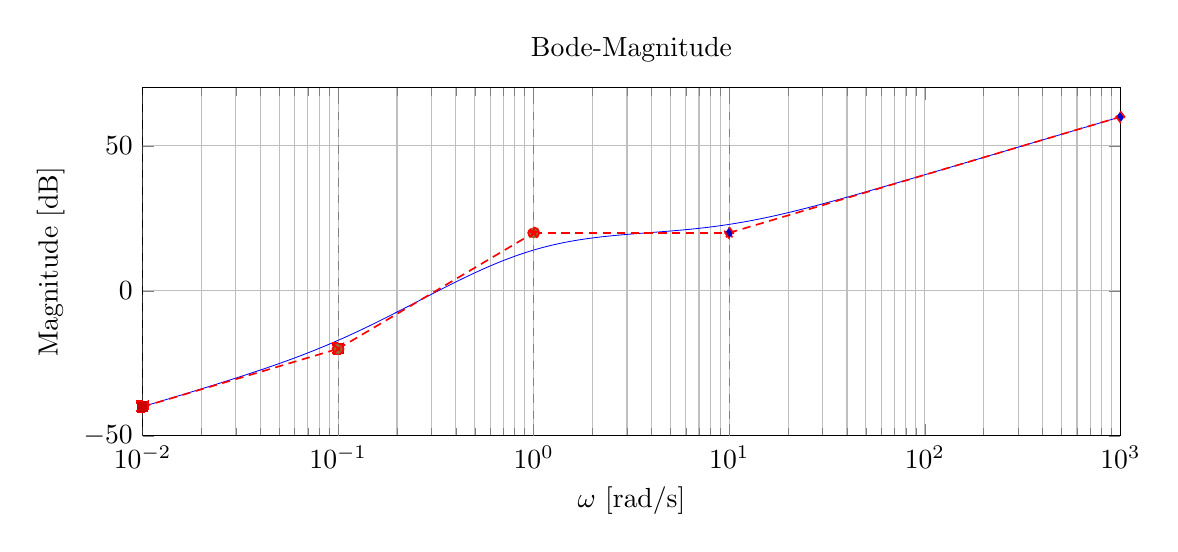
\begin{tikzpicture}
\begin{semilogxaxis}[
  width=14cm,height=6cm,
  xmin=1e-2,xmax=1e3,
  xlabel={$\omega$ [rad/s]},
  ylabel={Magnitude [dB]},
  grid=both,
  title={Bode-Magnitude}
]
\addplot[
  domain=1e-2:1e3,
  samples=800,
  mark=none,
  line width=0.3pt,
  blue
] {20*ln(x)/ln(10)
   +20*ln(sqrt(1 + (x/0.1)^2))/ln(10)
   +20*ln(sqrt(1 + (x/10)^2))/ln(10)
   -40*ln(sqrt(1 + x^2))/ln(10)};
\addplot+[domain=1e-2:1e-1,samples=2,dashed,dash pattern=on 3pt off 2pt,line width=0.6pt,red] {20*ln(x)/ln(10)};
\addplot+[domain=1e-1:1,samples=2,dashed,dash pattern=on 3pt off 2pt,line width=0.6pt,red] {40*ln(x)/ln(10) + 20};
\addplot+[domain=1:1e1,samples=2,dashed,dash pattern=on 3pt off 2pt,line width=0.6pt,red] {20};
\addplot+[domain=1e1:1e3,samples=2,dashed,dash pattern=on 3pt off 2pt,line width=0.6pt,red] {20 + 20*ln(x/10)/ln(10)};
\draw[gray,dashed] (rel axis cs:0,0) -- (rel axis cs:0,1);
\draw[gray,dashed] (axis cs:0.1,\pgfkeysvalueof{/pgfplots/ymin}) -- (axis cs:0.1,\pgfkeysvalueof{/pgfplots/ymax});
\draw[gray,dashed] (axis cs:1,\pgfkeysvalueof{/pgfplots/ymin}) -- (axis cs:1,\pgfkeysvalueof{/pgfplots/ymax});
\draw[gray,dashed] (axis cs:10,\pgfkeysvalueof{/pgfplots/ymin}) -- (axis cs:10,\pgfkeysvalueof{/pgfplots/ymax});
\node[gray,anchor=south east] at (axis cs:0.1,\pgfkeysvalueof{/pgfplots/ymax}) {\scriptsize Nullstelle $\omega_z=0.1$ (RHP)};
\node[gray,anchor=south east] at (axis cs:1,\pgfkeysvalueof{/pgfplots/ymax}) {\scriptsize Pol $\omega_p=1$ (doppelt)};
\node[gray,anchor=south east] at (axis cs:10,\pgfkeysvalueof{/pgfplots/ymax}) {\scriptsize Nullstelle $\omega_z=10$};
\end{semilogxaxis}
\end{tikzpicture}
\vspace{6mm}
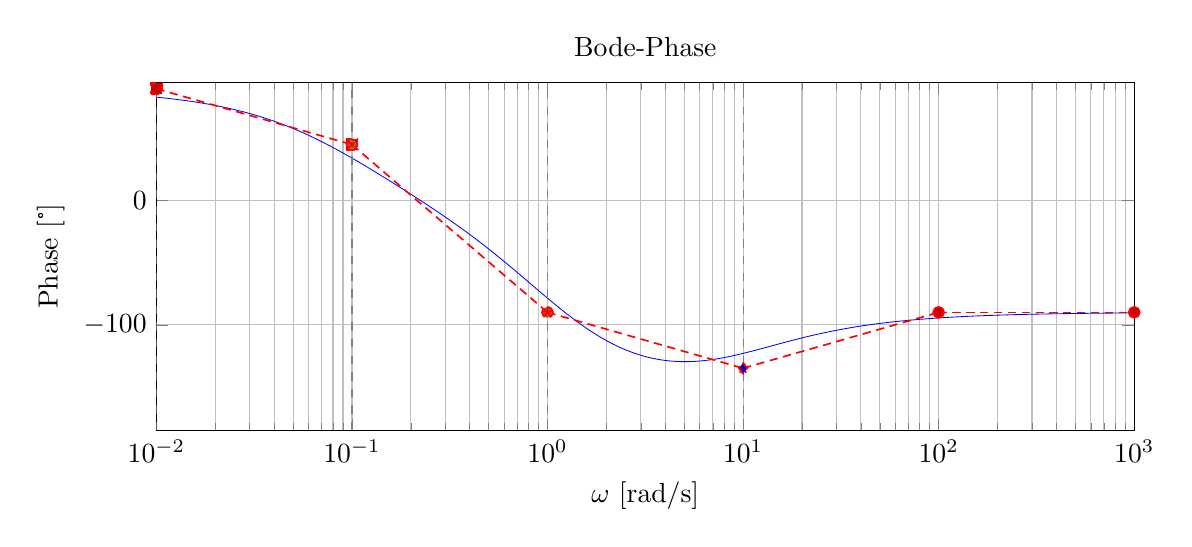
\begin{tikzpicture}
\begin{semilogxaxis}[
  width=14cm,height=6cm,
  xmin=1e-2,xmax=1e3,
  ymin=-185,ymax=95,
  xlabel={$\omega$ [rad/s]},
  ylabel={Phase [°]},
  grid=both,
  title={Bode-Phase}
]
\addplot[
  domain=1e-2:1e3,
  samples=800,
  mark=none,
  line width=0.3pt,
  blue
] {90 - atan(x/0.1) + atan(x/10) - 2*atan(x)};
\addplot+[domain=1e-2:1e-1,samples=2,dashed,dash pattern=on 3pt off 2pt,line width=0.6pt,red] {45 - 45*ln(x/0.1)/ln(10)};
\addplot+[domain=1e-1:1e0,samples=2,dashed,dash pattern=on 3pt off 2pt,line width=0.6pt,red] {45 - 135*ln(x/0.1)/ln(10)};
\addplot+[domain=1e0:1e1,samples=2,dashed,dash pattern=on 3pt off 2pt,line width=0.6pt,red] {-90 - 45*ln(x)/ln(10)};
\addplot+[domain=1e1:1e2,samples=2,dashed,dash pattern=on 3pt off 2pt,line width=0.6pt,red] {-135 + 45*ln(x/10)/ln(10)};
\addplot+[domain=1e2:1e3,samples=2,dashed,dash pattern=on 3pt off 2pt,line width=0.6pt,red] {-90};
\draw[gray,dashed] (rel axis cs:0,0) -- (rel axis cs:0,1);
\draw[gray,dashed] (axis cs:0.1,\pgfkeysvalueof{/pgfplots/ymin}) -- (axis cs:0.1,\pgfkeysvalueof{/pgfplots/ymax});
\draw[gray,dashed] (axis cs:1,\pgfkeysvalueof{/pgfplots/ymin}) -- (axis cs:1,\pgfkeysvalueof{/pgfplots/ymax});
\draw[gray,dashed] (axis cs:10,\pgfkeysvalueof{/pgfplots/ymin}) -- (axis cs:10,\pgfkeysvalueof{/pgfplots/ymax});
\node[gray,anchor=south east] at (axis cs:0.1,\pgfkeysvalueof{/pgfplots/ymax}) {\scriptsize Nullstelle $\omega_z=0.1$ (RHP)};
\node[gray,anchor=south east] at (axis cs:1,\pgfkeysvalueof{/pgfplots/ymax}) {\scriptsize Pol $\omega_p=1$ (doppelt)};
\node[gray,anchor=south east] at (axis cs:10,\pgfkeysvalueof{/pgfplots/ymax}) {\scriptsize Nullstelle $\omega_z=10$};
\end{semilogxaxis}
\end{tikzpicture}
\end{center}
\newpage
\subsection{Erklärung}
\vspace{5mm}
\begin{description}[leftmargin=1.2em,labelsep=.6em,font=\bfseries]
\item[Schritt 1] Struktur und Startverhalten: $H(s)=\dfrac{s(0.1-s)(s+10)}{(s+1)^2}$. Für $\omega\ll0.1$ gilt $|H(\j\omega)|\approx \omega\cdot 0.1\cdot 10/1=\omega$ $\Rightarrow$ Startsteigung $+20\,\mathrm{dB/dec}$; Startphase aus $\j\omega$ ist $\approx+90^\circ$ (keine Übergänge aktiv).
\item[Schritt 2] RHP-Nullstelle bei $\omega_z=0.1\,\mathrm{rad/s}$: Magnitude-Beitrag wie LHP-Nullstelle $\Rightarrow$ zusätzlicher Anstieg $+20\,\mathrm{dB/dec}$ ab $\omega=0.1$; Phase hingegen fällt nicht-minimumphasig um $90^\circ$ über $\omega\in[0.01,1]$ (Geradennäherung: $45^\circ-45^\circ\log_{10}(\omega/0.1)$ bis $45^\circ-135^\circ\log_{10}(\omega/0.1)$).
\item[Schritt 3] Doppelpol bei $\omega_p=1\,\mathrm{rad/s}$ und LHP-Nullstelle bei $\omega_z=10\,\mathrm{rad/s}$: Der Doppelpol reduziert die Slope um $-40\,\mathrm{dB/dec}$ $\Rightarrow$ Netto $0\,\mathrm{dB/dec}$ in $[1,10]$ (Betrag $\approx20\,\mathrm{dB}$ als Geraden-Niveau); die LHP-Nullstelle hebt ab $\omega=10$ die Slope wieder auf $+20\,\mathrm{dB/dec}$. Phasenbild: der Doppelpol liefert insgesamt $-180^\circ$ über $\omega\in[0.1,10]$; die LHP-Nullstelle addiert $+90^\circ$ über $\omega\in[1,100]$. Daraus resultieren die roten Segmente: $+90^\circ\to+45^\circ$ ($[0.01,0.1]$), weiter bis $\approx-90^\circ$ ($[0.1,1]$), in $[1,10]$ Abfall bis $\approx-135^\circ$, anschließend Anstieg zurück gegen $\approx-90^\circ$ für $\omega\gg100$.
\end{description}

\vspace{0.5cm}
\medskip
\noindent\textbf{Stückweise Näherung}
\[
|H(\j\omega)|_{\mathrm{dB}}\approx
\begin{cases}
20\log_{10}\omega,& \omega\ll0.1,\\[4pt]
40\log_{10}\omega+20,& 0.1\ll\omega\ll1,\\[4pt]
20,& 1\ll\omega\ll10,\\[4pt]
20+20\log_{10}(\omega/10),& \omega\gg10,
\end{cases}
\qquad
\]
\newpage